\section{SCR-ASC System Dynamics Under Catalyst Saturation}
%==
The SCR-ASC subsystem in the diesel engine aftertreatment systems involves reacting flow over a catalyst that
adsorbs ammonia from urea decomposition. The reaction kinetics start with the decomposition of urea into ammonia
followed by its adsorption onto the surface of the catalyst. The $\nox$ entering the chamber is reduced by this adsorbed
ammonia. The Eley-Rideal reaction mechanism \cite{prins2018eley}, \cite{yuan2015diesel}, \cite{hsieh2011development},
\cite{nova2014urea} is considered for modeling the SCR reaction kinetics, where ($\nox$), and
the other is adsorbed on the catalyst surface $(\ammonia)$. Reference~\cite{nova2014urea} lists all the reactions that take place
inside the SCR-ASC chamber. Ammonia oxidation (AMOX) happens on the surfaces of both the SCR and the ASC
catalysts, but the SCR catalyst favors $\nox$ reduction while the ASC is specifically designed for ammonia oxidation.
In order to keep the model order reasonably low and parameters identifiable, only the following three prominent reactions \cite{devarakonda2008adequacy},\cite{hsieh2011development} are considered:
\begin{enumerate}
    \item Standard SCR reaction:
    \begin{align}
        4 \ammonia ^{ads} + 4 \text{NO} + \oxygen &\xrightarrow[]{k_{scr}} 4 \nitrogen + 6 \water \label{eqn::std_scr}
    \end{align}
    \item Ammonia Oxidation:
    \begin{align}
        4 \ammonia^{ads} + 3 \oxygen &\xrightarrow[]{k_{oxi}} 2 \nitrogen + 6 \water \label{eqn::amox}
    \end{align}
    \item Ammonia Adsorption/Desorption:
        \begin{align}
            \ammonia + \Theta_{free} &\xrightleftharpoons[k_{des}]{k_{ads}} \ammonia^{ads}
            \label{eqn::ads}
        \end{align}
\end{enumerate}
%==
This aggregation of reactions results in errors in parameter estimates; specifically, parameters containing the rate
constant for the $\nox$ reduction $\lr{k_{scr}}$ have higher (bounded) uncertainty because they become dependent on the
nitrogen selectivity of the AMOX reaction \cite{jain2023diagnostics}.
%=======================================================================================================================
\begin{figure}[ht]
    \centering
    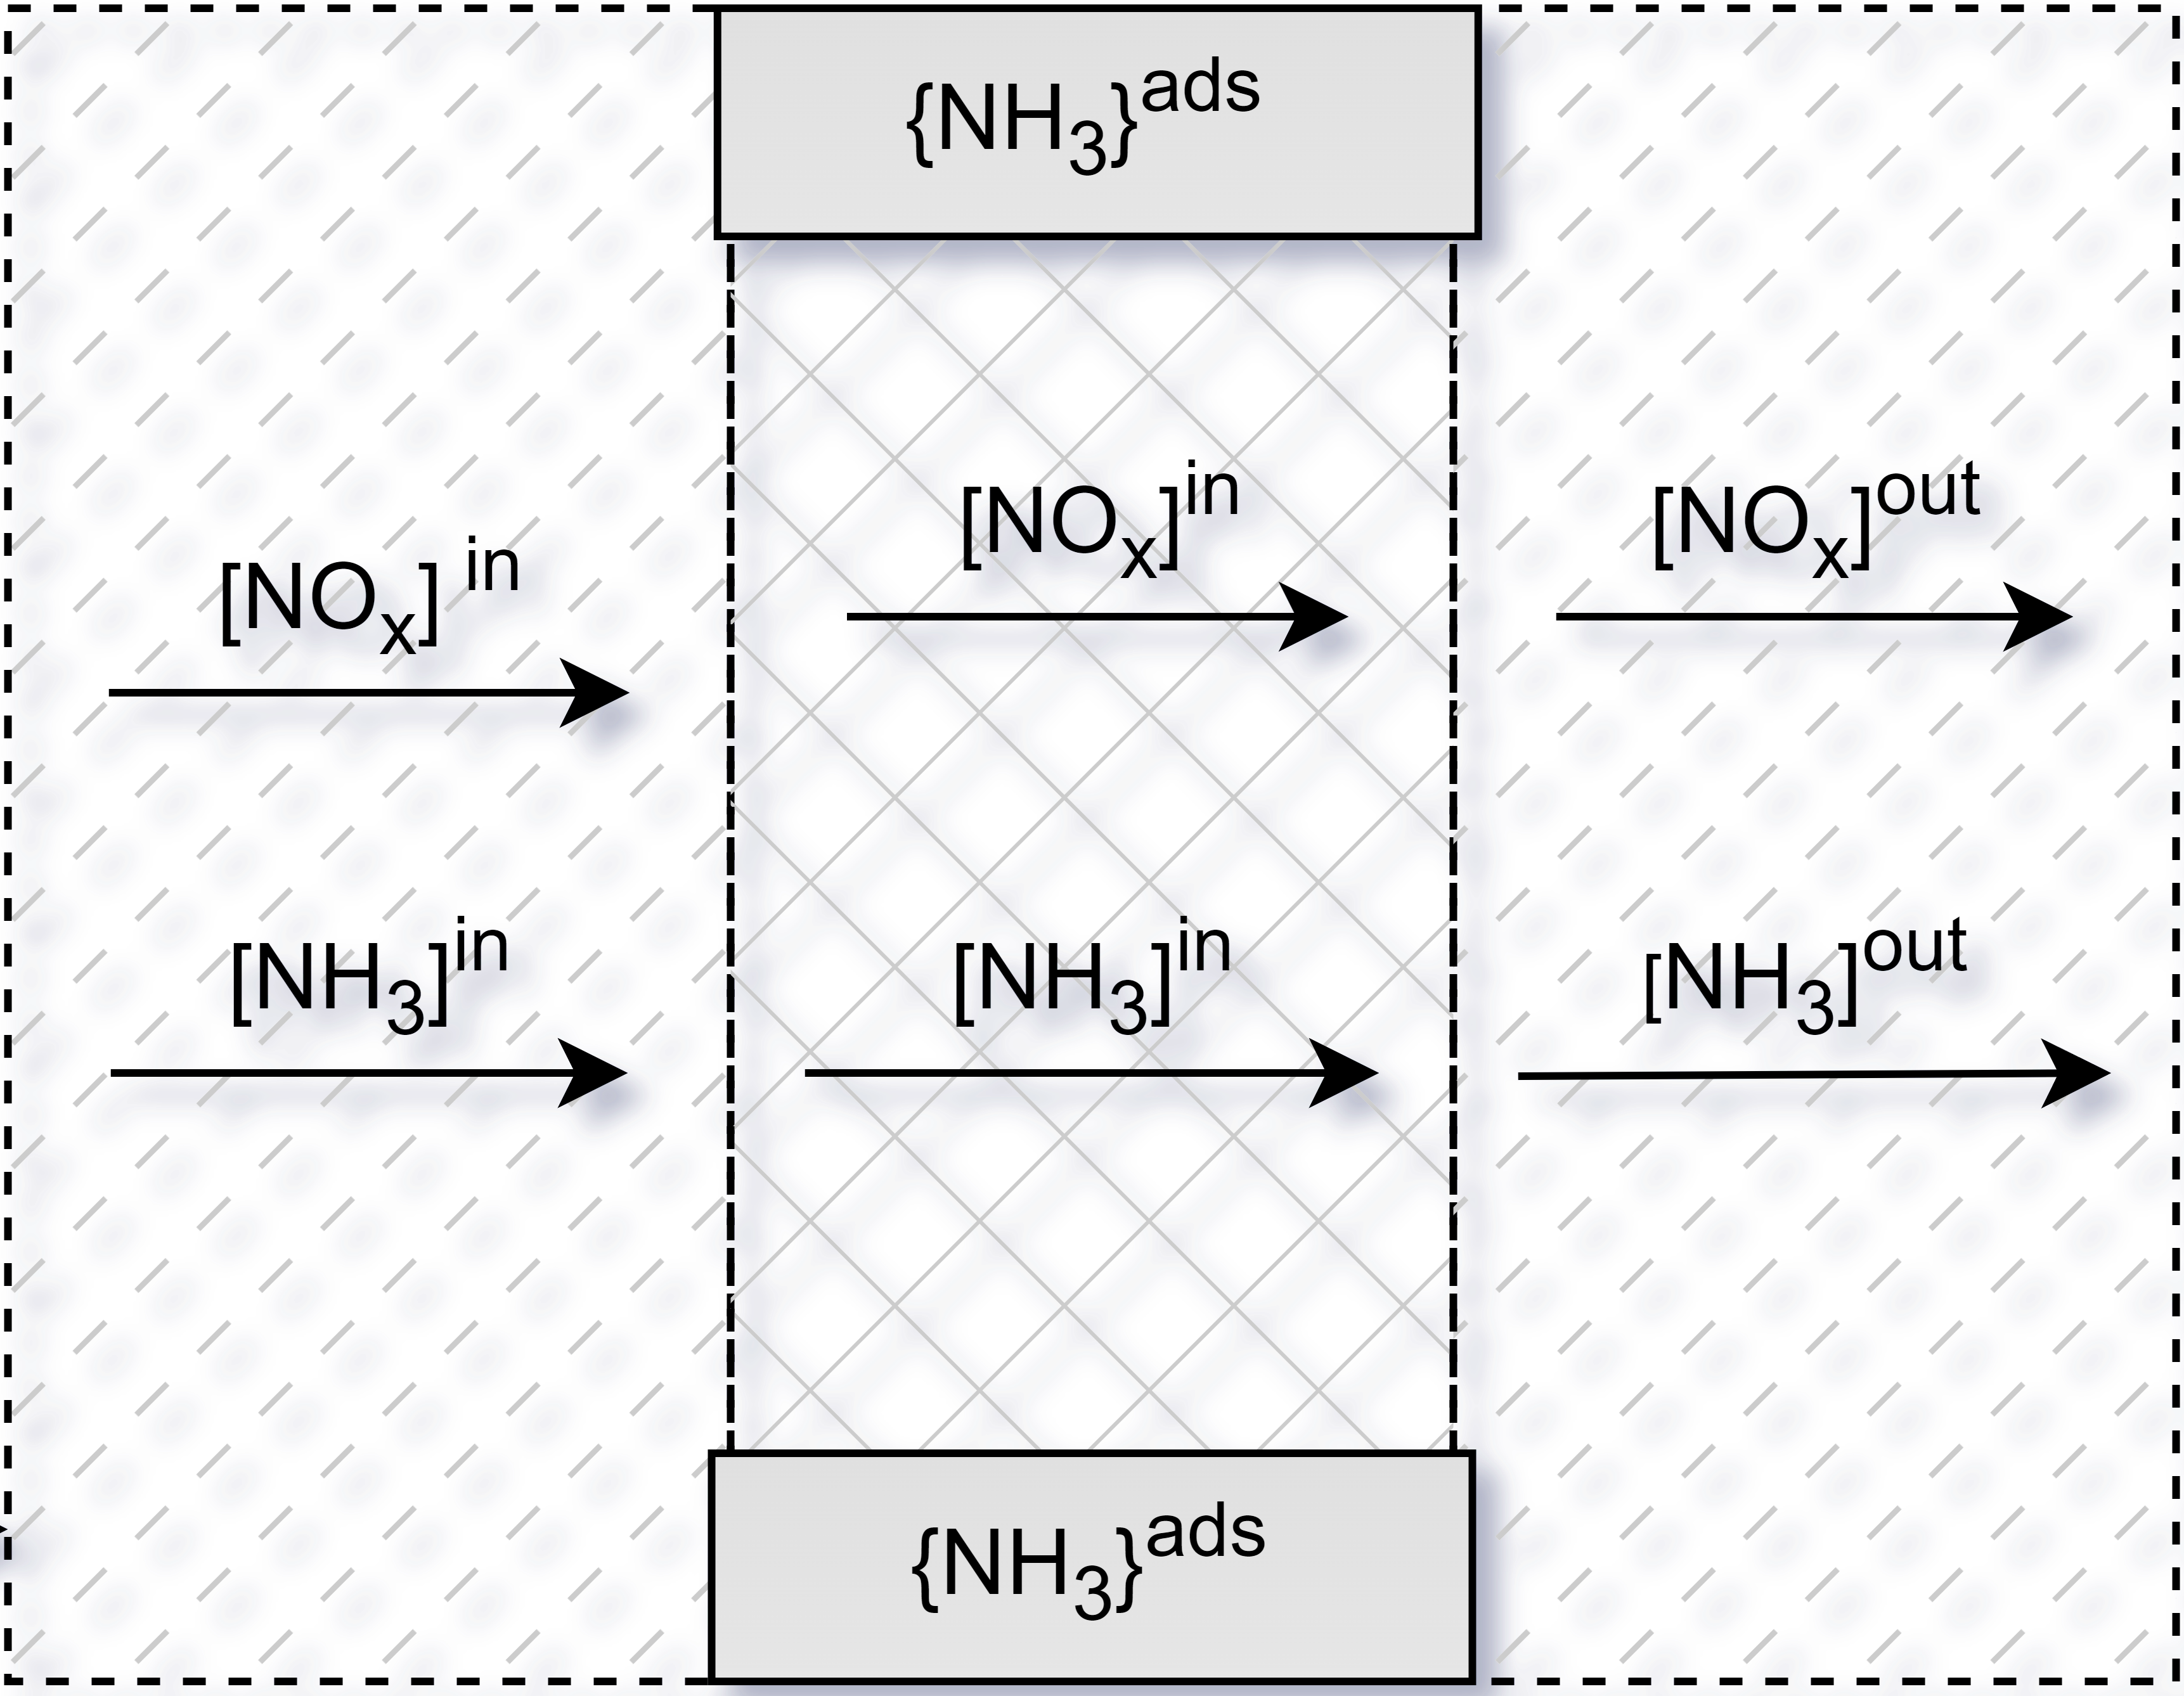
\includegraphics[width=0.3\textwidth]{figs/2_mdl/plug_flow_discrete.png}
    \caption{Control volume in plug flow reaction}
    \label{fig:plug-flow}
\end{figure}
%===
\input{secs/2-subs/2-0-sat_NOx_deriv.tex}
%===
\input{secs/2-subs/2-1-relative_response.tex}
%===
%===
\subsection{$\nox$ sensor cross-sensitivity}
Commercial $\nox$ sensors are cross-sensitive to tailpipe ammonia. Figure~\ref{fig::cross_sensitivity} shows the effect of cross-sensitivity on commercial $\nox$ sensors due to tailpipe ammonia. When the tailpipe ammonia is greater than a threshold value, the $\nox$ sensor output is corrupted, as shown in the plots where the $\nox$ sensor measurement is significantly higher than the FTIR measurement, which can be considered the true value. The resulting
error is modeled as a function of ammonia concentration and a temperature-dependent cross-sensitivity factor $\chi(T)$.
This introduces a non-negative directional error $\lr{\varepsilon_\chi= \chi\lr{T(k)} \times \con{\ammonia}^{out}\geq 0}$
into the tailpipe $\nox$ measurement $y_1$. Accordingly, when the $\nox$ reduction in a time step is calculated from
sensor measurements, $y_1(k) = x_1(k) + \varepsilon_{\chi}(k)$, the estimated quantity is less than the actual $\nox$
reduction:
\begin{align}
        \eta_y(k) &= u_1(k-1) - y_1(k) =  \eta(k) - \varepsilon_\chi(k) \leq \eta(k) \label{eqn::cross_meas}
\end{align}
Thus, the bounding condition on the saturated system's response (\ref{eqn::eta_bound}) remains valid when the $\nox$ reduction during the time step is estimated from the $\nox$ sensor measurements:
\begin{align}
        \eta_{sat}(k) &\geq \eta(k) = \eta_y(k) + \varepsilon_\chi(k) \geq \eta_y(k) \label{eqn::eta_y_bound}
\end{align}
%===
\begin{figure}[ht]
        \centering
        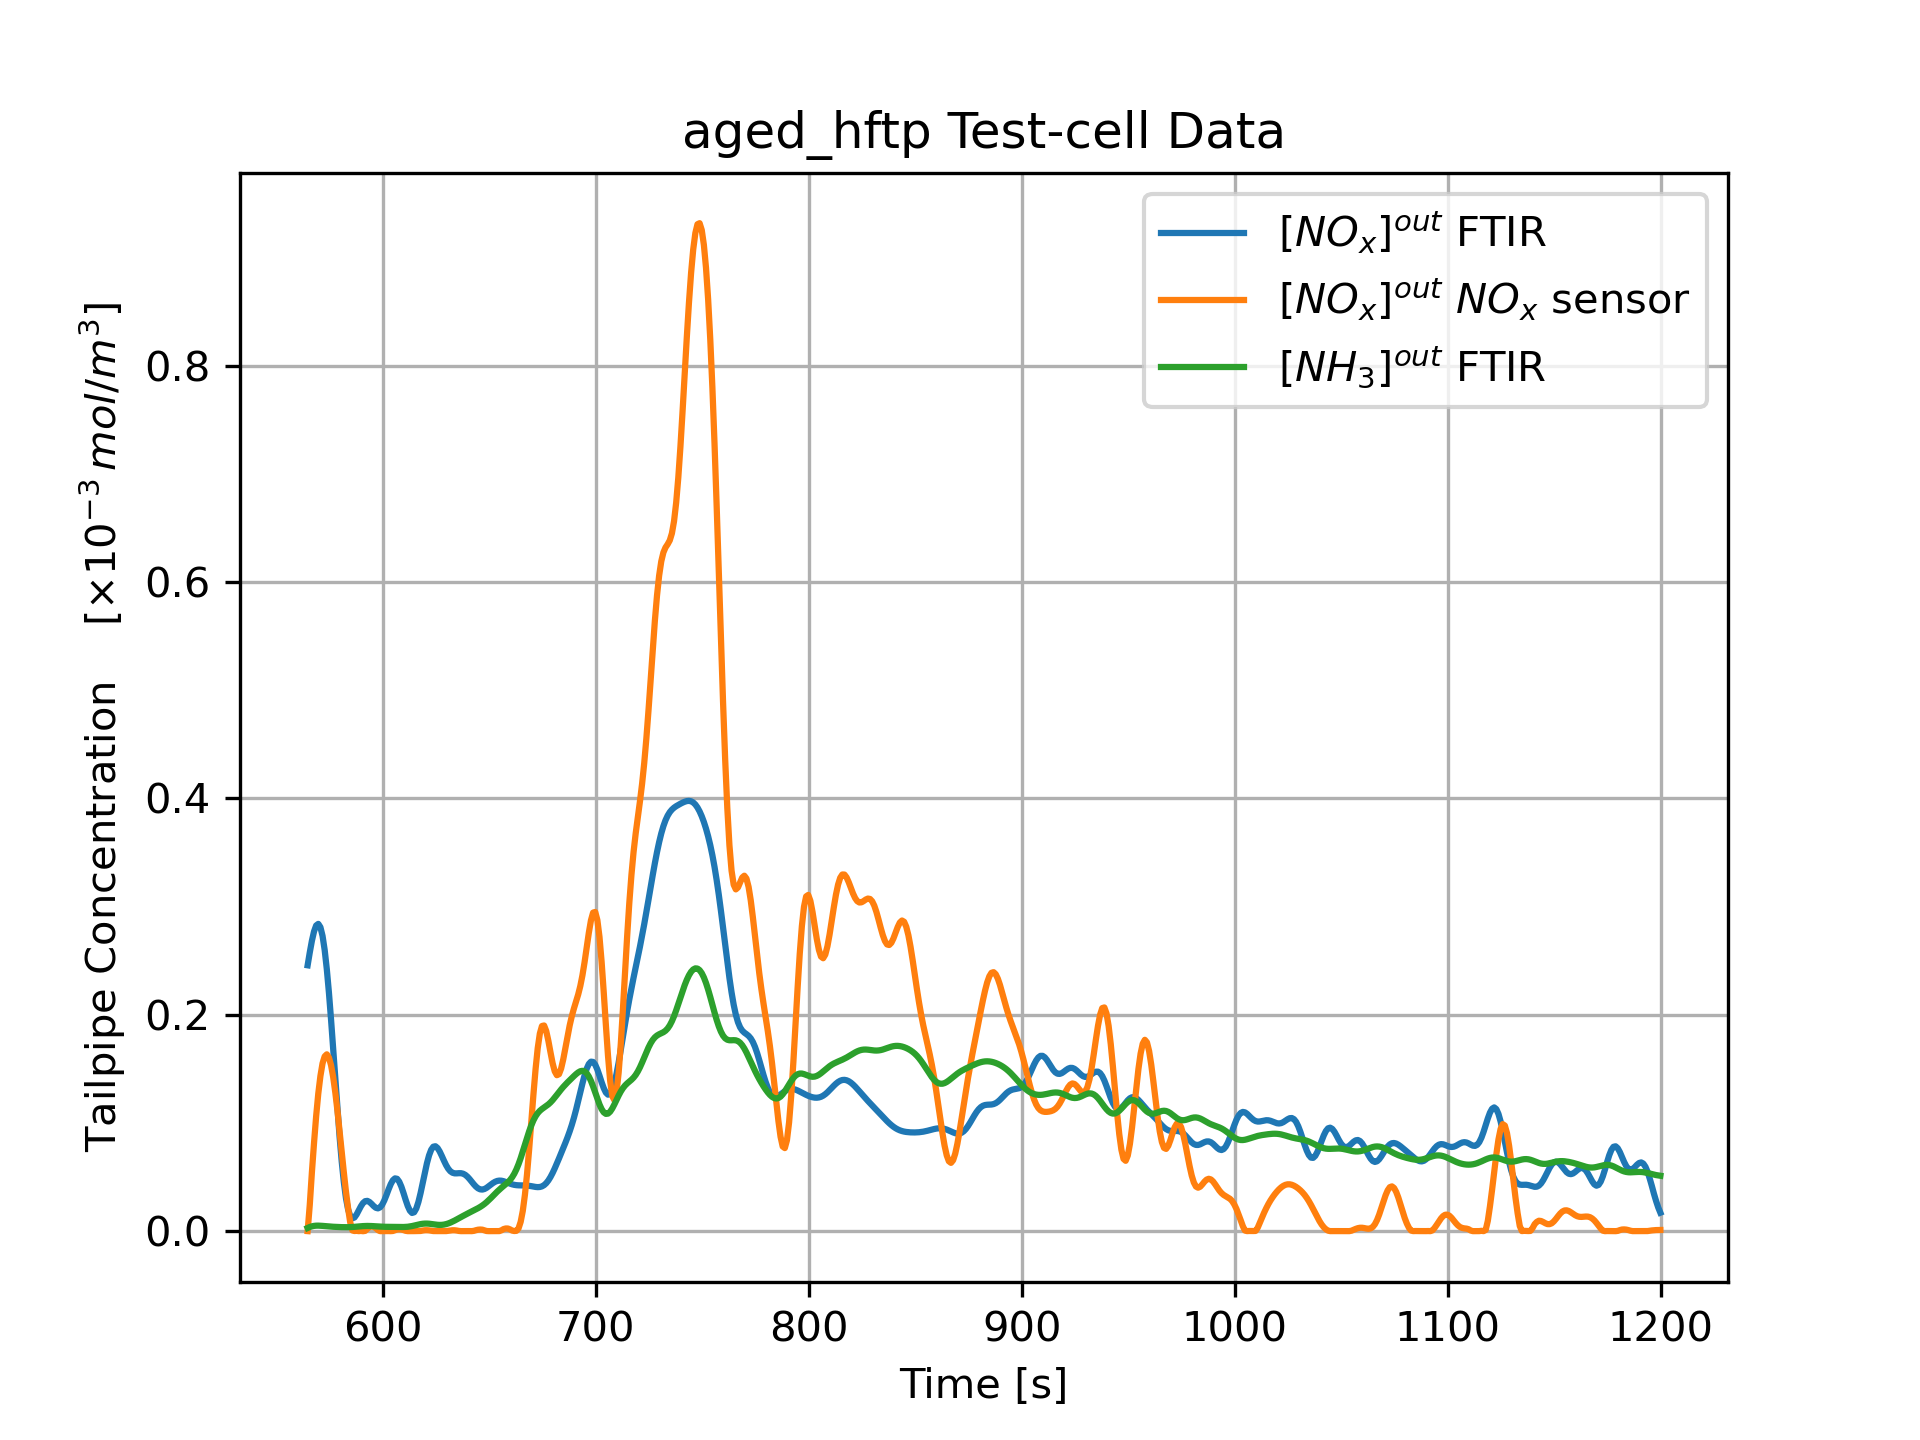
\includegraphics[width=\figWidth]{./figs/2_mdl/cross_aged_hftp.png}
        \caption{$\nox$ sensor cross-sensitivity to tailpipe ammonia}
        \label{fig::cross_sensitivity}
\end{figure}
% The FTIR sensor also has a bias that is directional. Similar arguments as above can be made for the validity of the
% bounding condition.

